\section{}
\textit{Integrate eq. (2) over the internal control volumes (2 - 3) using control volume 2 as a representative volume. Assume constant cross section value $S = 1$.}
\begin{figure}[H]
    \centering
    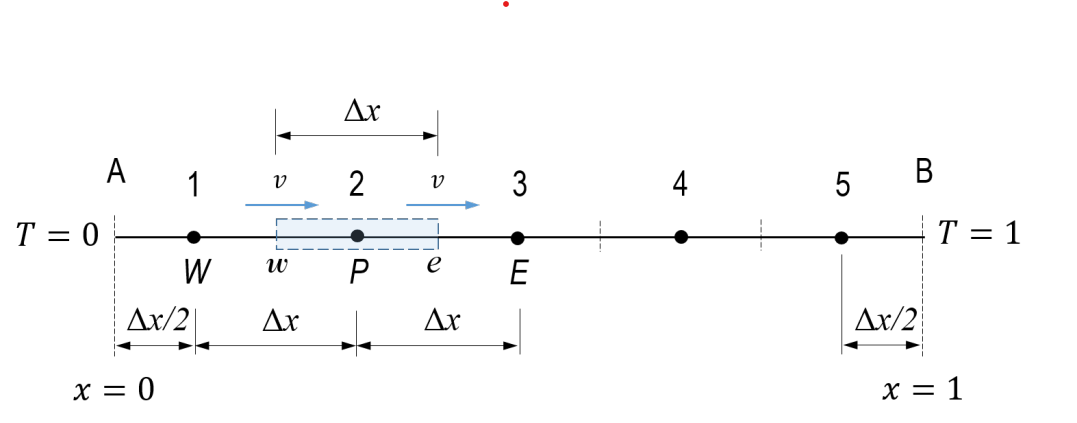
\includegraphics[width=0.8\textwidth]{Questions/Figures/Simulation Domain Mesh.png}
    \caption{Simulation Domain Mesh}
    \label{fig:mesh}
\end{figure}

Eq. 2 is given by:
\begin{align*}
    \frac{d \hat{T}}{dx} &= \frac{d}{dx}\left(\frac{1}{\text{Pe}}\frac{d \hat{T}}{dx}\right)
\end{align*}
Then integrating over the control volume,
\begin{align*}
    \int_{\Delta x} \frac{d \hat{T}}{dx} S dx &= \int_{\Delta x} \frac{d}{dx}\left(\frac{1}{\text{Pe}} \frac{d \hat{T}}{dx}\right) S dx \\
    \hat{T} \bigg|_{w}^{e} &= \left(\frac{1}{\text{Pe}} \frac{d \hat{T}}{dx}\right) \bigg|_{w}^{e} 
\end{align*}
Then,
\begin{align*}
    \Aboxed{\underbrace{\hat{T}_e - \hat{T}_w}_{\text{Convective}} &= \underbrace{\frac{1}{\text{Pe}} \left[\frac{d \hat{T}}{dx}\right]_e - \frac{1}{\text{Pe}} \left[\frac{d \hat{T}}{dx}\right]_w}_{\text{Diffusive}}}
\end{align*}

